\documentclass[tikz,border=2mm]{standalone}
\usepackage{pgfplots, caption}
\begin{document}
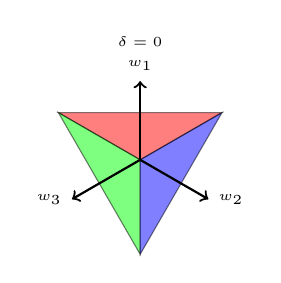
\begin{tikzpicture}
    \node at (0,1.5) {\tiny $\delta = 0$};

    \filldraw[fill=red, opacity=0.5] (0,0) -- (30:1.2) -- (150:1.2) -- (0,0);
    \filldraw[fill=green, opacity=0.5] (0,0) -- (150:1.2) -- (-90:1.2) -- (0,0);
    \filldraw[fill=blue, opacity=0.5] (0,0) -- (-90:1.2) -- (30:1.2) -- (0,0);

    \draw[->, thick] (0,0) -- (90:1) node [above] {\tiny $w_{1}$};
    \draw[->, thick] (0,0) -- (330:1) node [right] {\tiny $w_{2}$};
    \draw[->, thick] (0,0) -- (210:1) node [left] {\tiny $w_{3}$};
\end{tikzpicture}
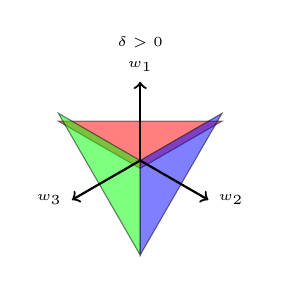
\begin{tikzpicture}
    \node at (0,1.5) {\tiny $\delta > 0$};

    \filldraw[fill=red, opacity=0.5, shift={(0,-0.1)}] (0,0) -- (30:1.2) -- (150:1.2) -- (0,0);
    \filldraw[fill=green, opacity=0.5] (0,0) -- (150:1.2) -- (-90:1.2) -- (0,0);
    \filldraw[fill=blue, opacity=0.5] (0,0) -- (-90:1.2) -- (30:1.2) -- (0,0);

    \draw[->, thick] (0,0) -- (90:1) node [above] {\tiny $w_{1}$};
    \draw[->, thick] (0,0) -- (330:1) node [right] {\tiny $w_{2}$};
    \draw[->, thick] (0,0) -- (210:1) node [left] {\tiny $w_{3}$};
\end{tikzpicture}

\end{document}
